\documentclass[
  html5,
  mathml,
  use filename
]{internet}

\imode<doc>{
  \usepackage{amsmath}
  \usepackage{amsthm}
  \usepackage{mymacros}

  \usepackage{tikz}
  \usetikzlibrary{matrix}
}

\imode<text>{
  \newtheorem{exercise}{Exercise}
  }

\addcss{
  .hline, .vline {
    border-collapse: collapse;
  }
  
  .hline td:first-child {
    border-right: solid black 1pt;
  }

  .vline tr:first-child {
    border-bottom: solid black 1pt;
  }
}

\usepackage{tutorial}
\usepackage{hyperref}

%\setLocation{file}

\title{A Little Excursion in Number Theory}
\date{\today}

\begin{document}
\maketitle
\tableofcontents

\section{Introduction}

\emph{Number Theory} is that part of mathematics that studies the properties of numbers.
At its core lie the prime numbers.
Starting with simple results like the \emph{prime decomposition}, and simple algorithms like \emph{Euclid's algorithm}, Number Theory builds up to ideas that underpin the security of the internet.

\section{Clock Arithmetic}

The key idea of clock arithmetic is to do your arithmetic as if on a clock face.
When you go past \(12\), you ``wrap around''.
Thus \(13\) becomes \(1\), \(14\) becomes \(2\), and so on.
In \emph{clock arithmetic}, then, \(2 \times 7 = 14\) which becomes \(2\).
Thus we might write \(2 \times 7 =_{\mathrm{c a}} 2\) where the subscript stands for ``clock arithmetic''.

There's one slight difference with clock arithmetic in mathematics: we use \(0\) instead of \(12\).
Thus our clock face starts at \(0\) and ends at \(11\).
So \(2 \times 6 =_{\mathrm{c a}} 0\).

We can also generalise to different clocks with different numbers.
We could imagine a clock with only four numbers: \(0,1,2,3\).
On this clock, we would have \(3 \times 3 = 9 =_{\mathrm{c a}} 1\) (since we wrap around twice).

Our notation gets a bit unwieldy here since it ought to record the ``clock number''.
The proper notation is to write:
%
\begin{align*}
2 \times 7 &\equiv 2 \mod 12 \\
2 \times 6 &\equiv 0 \mod 12 \\
3 \times 3 &\equiv 1 \mod 4
\end{align*}
%
We read this as, for example, ``\(2\) times \(7\) is equivalent to \(2\) modulo \(12\)''.

As we're using correct notation, we should use correct terminology as well.
The topic is known as \emph{modular arithmetic}, not ``clock arithmetic'', and the clock number is known as the \emph{modulus}.

If you think what is going on when doing the ``wrap around'', we can add or subtract multiples of the \emph{modulus} without changing what it is equivalent to.
So two numbers, say \(a\) and \(b\), are \emph{equivalent modulo \(n\)} if \(n\) divides their difference, \(b - a\).

We'll assume that modular arithmetic \emph{works}.
That is, there's never any ambiguity in working out the value of an expression.

\section{Multiplication Tables}

In modular arithmetic, there are only a finite number of ``numbers''.
For example, with modulus \(4\) then every number is equivalent to one of \(0\), \(1\), \(2\), or \(3\).

This means that we can write out all the possible multiplications in a \emph{multiplication table}.
For example, here's the multiplication table with modulus \(4\):

\begin{center}
\imode
<doc>
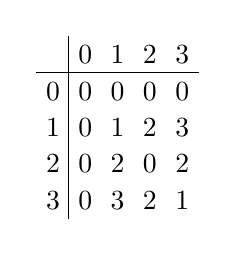
\begin{tikzpicture}
\matrix[matrix of math nodes,nodes in empty cells] (m) {
    & 0 & 1 & 2 & 3 \\
  0 & 0 & 0 & 0 & 0 \\
  1 & 0 & 1 & 2 & 3 \\
  2 & 0 & 2 & 0 & 2 \\
  3 & 0 & 3 & 2 & 1 \\
};
\draw (m-2-1.north west) -- (m-2-5.north east);
\draw (m-1-2.north west) -- (m-5-2.south west);
\end{tikzpicture}
\imode
<text>
\setClass{hline vline}
\begin{tabular}{ccccc}
& 0 & 1 & 2 & 3 \\
0 & 0 & 0 & 0 & 0 \\
1 & 0 & 1 & 2 & 3 \\
2 & 0 & 2 & 0 & 2 \\
3 & 0 & 3 & 2 & 1 
\end{tabular}
\imode
<all>
\end{center}

The row and column corresponding to \(0\) is a bit dull, so we'll leave that out and just write:

\begin{center}
\imode<doc>
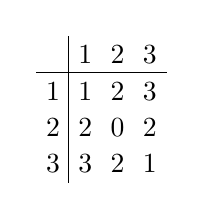
\begin{tikzpicture}
\matrix[matrix of math nodes,nodes in empty cells] (m) {
    &  1 & 2 & 3 \\
  1 &  1 & 2 & 3 \\
  2 &  2 & 0 & 2 \\
  3 &  3 & 2 & 1 \\
};
\draw (m-2-1.north west) -- (m-2-4.north east);
\draw (m-1-2.north west) -- (m-4-2.south west);
\end{tikzpicture}
\imode
<text>
\setClass{hline vline}
\begin{tabular}{cccc}
    &  1 & 2 & 3 \\
  1 &  1 & 2 & 3 \\
  2 &  2 & 0 & 2 \\
  3 &  3 & 2 & 1 \\
\end{tabular}
\imode
<all>
\end{center}

\begin{exercise}
\begin{enumerate}
\item Write out the multiplication table for a few moduli.
\item Some rows are ``special'' in that they have every number (other than \(0\)) on them.
What characterises these rows?
\item Are there any moduli where every row is ``special''?
\end{enumerate}
\end{exercise}

\section{Division}

Let's look at one of the ``special'' rows, for example the \(3\)--row in the multiplication table for \(4\).
Since each number appears there, we can say that for any number \(a\), there is some number \(b\) such that \(3 b \equiv a \mod 4\).

Now in normal arithmetic, we would say that if \(3 b = a\) then \(b = a/3\).
We don't have fractions in modular arithmetic, but we can still say that if \(3 b \equiv a \mod 4\) then there is some \(d\) such that \(b \equiv a d \mod 4\).

\begin{exercise}
For each \(a\), find \(d\) such that if \(3 b \equiv a \mod 4\) then \(b \equiv a d \mod 4\).
What do you notice?

What is \(3 d\)?
Is this a coincidence?
\end{exercise}

Hopefully you noticed that you got the same \(d\) each time.
In fact, in this case \(d = 3\).
It \emph{is} a coincidence that \(d = 3\) but not a coincidence that \(3 \times 3 \equiv 1 \mod 4\).

\begin{exercise}
Pick a ``special'' row in one of your other multiplication tables and repeat the above.

For a modulus where every row is special, write out a table pairing each number with its corresponding partner.
\end{exercise}

When we have this situation, we can ``undo'' multiplication.
For example, working modulo \(9\) (that is, with modulus \(9\)) then \(4\) has this property.
To undo multiplication by \(4\), we multiply by \(7\).
So \(7\) behaves like \(1/4\).
Another way of writing \(1/4\) is \(4^{-1}\) and we use this notation and refer to the \emph{reciprocal} of \(4\).
Thus: \(4^{-1} \equiv 7 \mod 9\).

Our conclusion is that for every ``special'' modulus, then every non-zero number has a reciprocal and so we can ``do division''.

\begin{exercise}
What about the non-special moduli?
Which numbers do not have reciprocals?
\end{exercise}

\section{Powers}

Let's move on to powers.
Just as with multiplication, we can do powers and write out a ``power table''.
Also just as with multiplication, it makes sense to ignore powers of \(0\) but we will include \(a^0 = 1\) as our first column.
We'll write it out up to \(a^{n-1}\), where \(n\) is our modulus.
Thus for \(4\) our ``power table'' looks like this:

\begin{center}
\imode<doc>
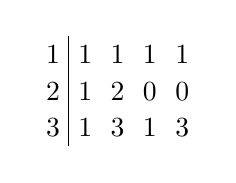
\begin{tikzpicture}
\matrix[matrix of math nodes,nodes in empty cells] (m) {
  1 & 1 & 1 & 1 & 1 \\
  2 & 1 & 2 & 0 & 0 \\
  3 & 1 & 3 & 1 & 3 \\
};
\draw (m-1-2.north west) -- (m-3-2.south west);
\end{tikzpicture}
\imode
<text>
\setClass{hline}
\begin{tabular}{ccccc}
  1 & 1 & 1 & 1 & 1 \\
  2 & 1 & 2 & 0 & 0 \\
  3 & 1 & 3 & 1 & 3 \\
\end{tabular}
\imode
<all>
\end{center}

\begin{exercise}
Write out the power table for a variety of moduli.
What special features do you notice?
\end{exercise}

In this case, only some moduli have ``special rows'' where every number appears, but even when some rows are ``special'' then not every row is.
A number \(a\) such that \(a^0\), \(a^1\), \(a^2\), etc.\ generates all the numbers is called a \emph{primitive root}.

\begin{exercise}
Find primitive roots for the first few moduli that have them.
\end{exercise}

\section{Cryptography}

At the heart of modern cryptography lies the ability to have a secret conversation even in the presence of eavesdroppers.
The key to this is that it is possible for two people to both know something \emph{without actually exchanging that information}.

Let's see how this works.
It is traditional for the two protagonists in cryptography to be called \emph{Alice} and \emph{Bob}.
Let's keep the traditions.

\begin{enumerate}
\item In plain sight of everyone, Alice and Bob pick a nice prime number, say \(p\), and a smaller number, say \(g\).
So everyone knows \(p\) and \(g\), including any eavesdroppers.

\item Alice and Bob then each choose another number \emph{in secret}.

So Alice chooses a number, say \(n\), and Bob chooses a number, say \(m\).

\item Alice and Bob each calculates the corresponding power of \(g\) modulo \(p\).

So Alice calculates \(g^n \mod p\) and Bob \(g^m \mod p\).
Let's call these \(a\) and \(b\) respectively.

\item These two numbers are exchanged, again in plain sight.

\item Then Alice computes \(b^n \mod p\) and Bob computes \(a^m \mod p\).
The crucial fact is that these two produce exactly the same number, which is \(s = g^{m n} \mod p\).

\item Alice and Bob can then use this number in some secret code, and any eavesdropper doesn't know either \(m\) or \(n\) so can't figure out \(s\).
\end{enumerate}

Of course, given enough time and computing power, the evil eavesdropper could compute every single \(g^k \mod p\) and eventually figure out \(n\) and \(m\).
Looking at your ``power tables'', you should see that there is no particular pattern to the numbers \(g^k \mod p\) and so the eavesdropper would genuinely have to calculate them all.
There is no quick method.

In practice, the numbers chosen are big enough that this is practically impossible.

Thus Alice and Bob have agreed on a number, \(s\), without anyone else knowing what it is even though their entire conversation could be overheard.

\begin{exercise}
Carry out the exchange with a partner to agree on a ``secret number''.
\end{exercise}

\end{document}
